\hspace{0.6cm}Neutron stars are highly compacted core of a dead star, left behind as a remnant of supernova explosion. The pulsars are a unique type of neutron stars that emits beams of electromagnetic radiation out of its magnetic poles. The radiation can be detected from the Earth as blinking star through radio telescopes. The radiation is emitted in the periodic pattern so it appears as a pulsed emission of radiation. The discovery of pulsars was done by Jocelyin Bell a graduate student at Cambridge University in England in the year 1967 who was working under Antony Hewish \cite{AstronomyAndbeyond:1999}. She found out a peculiar pattern in the data in the form of regular pulses. This data was different from the radio signals of the celestial bodies that they detected earlier. At first, they thought that the signal is from some alien civilization so they named them as Little Green Men (LGM) but after few weeks they observed that there were three more objects in the other parts of the sky pulsing with different periods hence they dropped the name Little Green Men and renamed them as Pulsar.\\

Pulsars are among the strangest objects within the universe. Astronomers and scientists use pulsars as an instrument to detect gravitational waves. Pulsars are still found by using large radio telescopes. The largest radio telescope in the world is located at Arecibo in Puerto Rico. A telescope scans the entire sky and scientists look for objects that appear in and out. When a pulsar rotates, it produces detectable pattern of radio emission which is very precise and repeats periodically. Its maximum intensity rises and falls every 23 hours 56 minutes. Pulsars spin because the stars from which they are formed also rotate. The slowest pulsar ever detected spins on the order of one per second and the fastest pulsars can spin hundreds of times per second from earth, pulsars often look like flickering stars. On and off, on and off and they seem to blink with a regular rhythm. But the light waves from pulsars doesn't actually flicker or pulse. It radiates two steady, narrow beams of light in opposite direction. The light from the beam is steady and pulsars appear to flicker because they also spin for the same time. \cite{AstronomyAndbeyond:1999}\\

Pulsars are considered to be a great tool in determining the existence of gravitational waves.In 1974 the first evidence of gravitational waves was deduced through the motion of the double neutron star system PSRB1913+16  \cite{Linear}. In this system one of the star is a pulsar which emits electromagnetic pulses at radio frequencies precisely at regular intervals as it rotates. Russell Hulse and Joseph Taylor discovered this binary pulsars also noticed that the frequency of pulses shortened and the stars were gradually spiraling towards each other with an energy loss which is closely equal to the energy predicted to be radiated by gravitational waves. For this discovery, Hulse and Taylor were awarded the Nobel Prize in Physics 1993 \cite{Lommen_2015}. Further observations of the binary pulsar and other multiple systems also agree with the General theory of Relativity to high precision. This evidence of gravitational waves is considered as the first indirect evidence of gravitational waves. 
 
\begin{figure}[h]
    \centering
    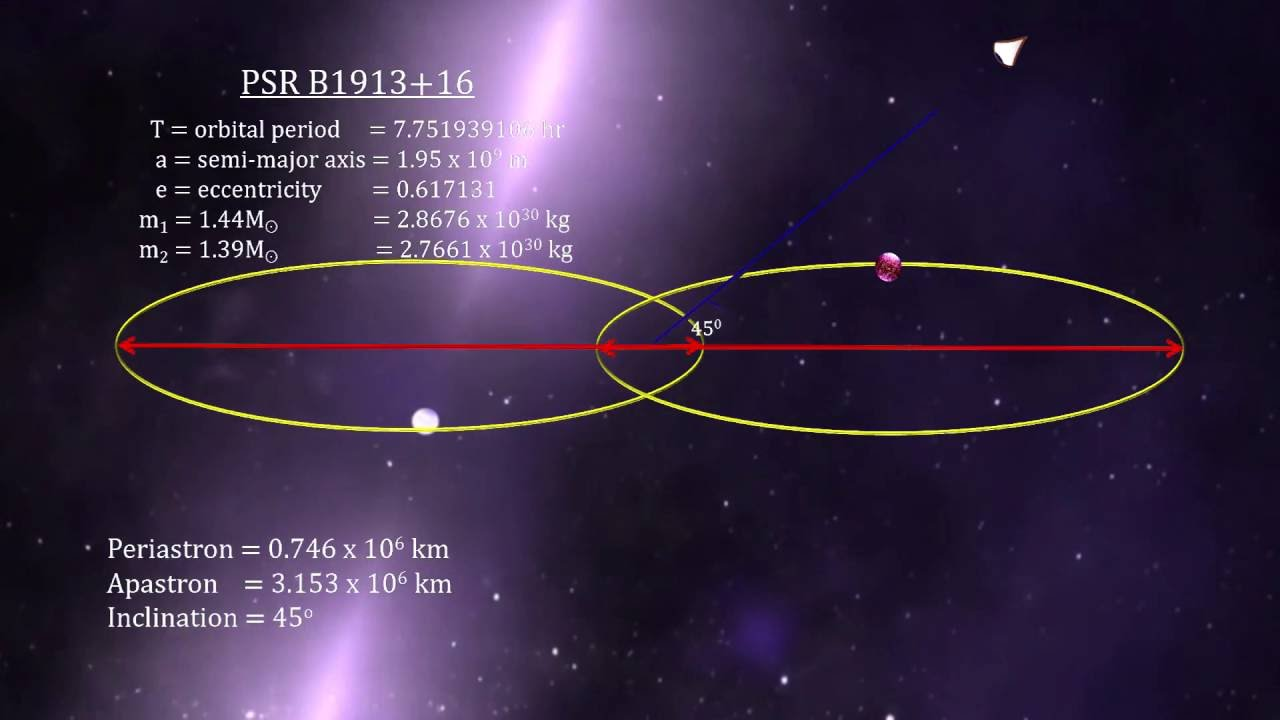
\includegraphics[scale=0.255]{images.tex/PSR-B191316.jpg}
    \caption{Binary pulsar PSR B1913+16. Source :- \href{https://www.astroblogs.nl/wp-content/uploads/2014/03/PSR-B191316.jpg}{Astroblogs.nl}}
\end{figure}

\pagebreak
